\documentclass{sbc2023}%
\usepackage{algorithm}
\usepackage{algpseudocode}
\usepackage{tikz} % Para desenhar o grafo
\usetikzlibrary{graphs, graphs.standard, quotes} 
\usepackage{booktabs} % Para tabelas profissionais
\usepackage{caption} % Para legendas

\usepackage{pgfplots}
\pgfplotsset{compat=1.18} % Garante a melhor renderização

% Tradução das palavras-chave para português
\algrenewcommand\algorithmicrequire{\textbf{Entrada:}}
\algrenewcommand\algorithmicensure{\textbf{Saída:}}
\algrenewcommand\algorithmicif{\textbf{se}}
\algrenewcommand\algorithmicthen{\textbf{então}}
\algrenewcommand\algorithmicelse{\textbf{senão}}
\algrenewcommand\algorithmicwhile{\textbf{enquanto}}
\algrenewcommand\algorithmicdo{\textbf{efetuar}}
\usepackage{graphicx}
%\usepackage[utf8]{inputenc}
\usepackage[misc,geometry]{ifsym} 
\usepackage{fontspec}
\usepackage{fontawesome}
\usepackage{academicons}
\usepackage{color}
\usepackage{hyperref} 
\usepackage{aas_macros}
\usepackage[bottom]{footmisc}
\usepackage{supertabular}
\usepackage{afterpage}
\usepackage{url}
\usepackage{pifont}
\usepackage{multicol}
\usepackage{multirow}
\usepackage{enumitem}
\usepackage{float}
\usepackage{listings} %\ Para códigos
% Importa as configurações do arquivo separado
% CoresCodigos.tex
\usepackage{listings}
\usepackage{xcolor}

\definecolor{corComentario}{rgb}{0.0, 0.5, 0.0}
\definecolor{corKeyword}{rgb}{0.0, 0.0, 1.0}
\definecolor{corString}{rgb}{0.63, 0.12, 0.09}
\definecolor{corFundo}{rgb}{0.95, 0.95, 0.92}
\definecolor{corNumero}{rgb}{0.5, 0.5, 0.5}

\lstset{
    backgroundcolor=\color{corFundo},
    commentstyle=\color{corComentario},
    % ... resto do seu código de configuração ...
    showstringspaces=false
}

\usepackage{xcolor} % Necessário se quiser colocar cores
\setcitestyle{square}

\definecolor{orcidlogo}{rgb}{0.37,0.48,0.13}
\definecolor{unilogo}{rgb}{0.16, 0.26, 0.58}
\definecolor{maillogo}{rgb}{0.58, 0.16, 0.26}
\definecolor{darkblue}{rgb}{0.0,0.0,0.0}
\hypersetup{colorlinks,breaklinks,
            linkcolor=darkblue,urlcolor=darkblue,
            anchorcolor=darkblue,citecolor=darkblue}
%\hypersetup{colorlinks,citecolor=blue,linkcolor=blue,urlcolor=blue}

%%%%%%% IMPORTANT: We disable hyperlinks by default with this line, to avoid the error "\pdfendlink ended up in different nesting level" while writing.
%\hypersetup{draft}

\jid{JBCS}
\jtitle{Trabalho Pratico 01, Teoria dos Grafos e Computabilidade, 2026}
\copyrightstatement{This work is licensed under a Creative Commons Attribution 4.0 International License}
\jyear{202X}


\title[TRABALHO PRÁTICO]{TRABALHO PRÁTICO}

%THE ORCID IS MANDATORY FOR EACH AUTHOR IN JBCS
\author[Viterbo et al. 202X]{

\affil{\textbf{Aisha Camille}~\href{https://orcid.org/0000-0002-7110-2026}{\textcolor{orcidlogo}{\aiOrcid}}~\textcolor{blue}{\faEnvelopeO}~~[~\textbf{Pontifícia Universidade Católica de Minas Gerais}~|\href{mailto:clodis.boscarioli@unioeste.br}{~\textbf{\textit{aisha.camille@sga.pucminas.br}}}~]}

\affil{\textbf{Iuri Saad}~\href{https://orcid.org/0000-0002-0339-6624}{\textcolor{orcidlogo}{\aiOrcid}}~\textcolor{blue}{\faEnvelopeO}~~[~\textbf{Pontifícia Universidade Católica de Minas Gerais}~|\href{mailto:viterbo@ic.uff.br}{~\textbf{\textit{saadiuri845@gmail.com}}}~]}

\affil{\textbf{Mateus Brant}~\href{https://orcid.org/0000-0003-3052-3016}{\textcolor{orcidlogo}{\aiOrcid}}~\textcolor{blue}{\faEnvelopeO}~~[~\textbf{Pontifícia Universidade Católica de Minas Gerais}~|\href{mailto:rpereira@inf.ufpr.br}{~\textbf{\textit{mateuscbcg@gmail.com}}}~]}



}

\begin{document}

\begin{frontmatter}
\maketitle

\begin{mail}
Ciências da Computação, Pontifícia Universidade Católica de Minas Gerais. 
\end{mail}


\begin{abstract}
\textbf{Resumo.~}
\noindent A analise do experimento a seguir sugerido pela aula de Teoria dos Grafos e Computabilidade, é focada na identificação de pontes. No trabalho foi utilizado o Método Tarjan e o método Naive em que testa a conectividade do grafo a pós a remoção de aresta. Além da identificação de pontes, o trabalho também tem como objetivo encontrar trajetos eurelianos em um grafo qualquer usando o Método fleury, registrando o tempo que o algoritmo leva para grafos de 100, 1000, 10000 e 100000 vertices.
\end{abstract}


\begin{keywords}
Grafos, Tarjan, Naive, Fleury, algoritmo, ponte
\end{keywords}

%\begin{license}
%Published under the Creative Commons Attribution 4.0 International Public License (CC BY 4.0)
%\end{license}

\end{frontmatter}


\section{Introdução}
\label{sec:intro}

Um dos objetivos do trabalho é identificação de pontes, a ponte em um grafo vai ser uma aresta em que se removida o grafo deixa de ser conexo, ou vai aumentar o número de componentes de um grafo~\citep{ref4}. E enquanto o outro objetivo, econtrar trajetos eurelianos,Um trajeto euleriano é um trajeto que passa por cada aresta de um grafo exatamente uma vez, Um ciclo euleriano é um trajeto euleriano que começa e termina no mesmo vértice, ou seja, um trajeto fechado. Um grafo vai ser dito eureliano se houver um ciclo eureliano. Um grafo é semi-euleriano se possuir um trajeto euleriano. Logo, um grafo euleriano é também semi-euleriano. Além das definições de trajetos e ciclos eurelianos, temos as condições necessárias para um grafo ser dito eureliano, como por exemplo segundo o Teorema de Euler, Um grafo conexo é euleriano se e somente se todos os seus vértices possuírem grau par, um grafo conexo semi-eureliano se poossuir exatamente dois vértices de grau ímpar, e um grafo conexo não eureliano se possuir mais de um vértice com grau ímpar.
O trabalho em questão exige a implementação de algoritmo Fleury (utilizado para identificar se um grafo é eureliano), utilizando os algoritmos de Tarjan e Naive para a detecção de pontes, foram testados em grafos de 10, 100, 10000 e 100000 vertices e registrado o tempo que cada algoritmo levou para fazer sua tarefa em cada grafo, buscando identificar a diferença de tempo médio de execução dos algoritmos enquanto o grafo cresce. ~\citep{slide}. 
\begin{figure}[H]
    \centering
    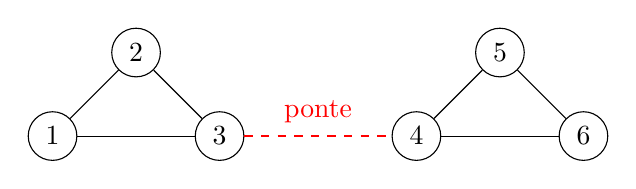
\begin{tikzpicture}[
        every node/.style={circle, draw, minimum size=0.6cm},
        node distance=1.5cm
    ]
        % Vértices
        \node (1) {1};
        \node (2) [above right of=1] {2};
        \node (3) [below right of=2] {3};
        \node (4) [right of=3, xshift=1cm] {4};
        \node (5) [above right of=4] {5};
        \node (6) [below right of=5] {6};

        % Arestas (Ciclo 1)
        \draw (1) -- (2);
        \draw (2) -- (3);
        \draw (3) -- (1);

        % Ponte
        \draw[thick, dashed, red] (3) -- node[above, draw=none, rectangle] {ponte} (4);

        % Arestas (Ciclo 2)
        \draw (4) -- (5);
        \draw (5) -- (6);
        \draw (6) -- (4);
    \end{tikzpicture}
    \caption{Exemplo de grafo com uma aresta de corte (ponte) ligando dois subgrafos.}
    \label{fig:exemplo_grafo}
\end{figure}

\section{Metodologia}

O projeto foi desenvolvido na linguagem Java, para a representação dos grafos, o grupo optou pela uso da lista de adjacência com o HashSet, a estrutura escolhida garante o acesso rápido a cada vértice e aos seus vizinhos, e também a remoção de arestas em tempo o(1), o que contrubuiu para a possibilidade do algoritmo de fleury~\citep{AlgoFleury} em grafos grandes, embora o tempo de execução para vértices de 100k tenha sido um desafio mesmo para a estrutura pensada em velocidade.

Os grafos considerados neste trabalho são simples, conexos e não direcionados, não possuindo laços nem arestas duplicadas. Essa definição é fundamental para a correta aplicação dos algoritmos analisados. Já que os mesmo são relacionados a propriedades eulerianas.

\subsection{Estrutura de dados}

A escolha da estrutura de dados para representar os grafos foi um fator crítico para a viabilidade e eficiência do projeto. Optou-se pela utilização de listas de adjacência implementadas com HashSet, conforme definido na classe Grafo.
A estrutura principal é representada por:

\begin{lstlisting}[language=C]
    HashSet<Integer>[] adj;
\end{lstlisting}

Nesse modelo, cada posição do array corresponde a um vértice, e o HashSet associado armazena seus vértices adjacentes. Essa escolha não foi arbitrária: ela oferece um equilíbrio entre eficiência de acesso e flexibilidade estrutural.

\subsubsection{Justificativa da escolha}

O uso de HashSet garante que operações fundamentais, como:
\begin{itemize}
    \item Verificação da existência de uma aresta (\lstinline|hasEdge|);
    \item Inserção de uma nova aresta (\lstinline|addEdge|).
\end{itemize}

Sejam executadas cm complexidade média O(1).
Essa característica foi essencial para o desempenho, especialmente considerando a aplicação do Algoritmo de Fleury~\citep{AlgoFleury}, que demanda múltiplas verificações de arestas e, potencialmente, simulações de remoção durante a identificação de pontes.

Em grafos de grande escala (até 100.000 vértices), estruturas menos eficientes, como listas encadeadas simples ou matrizes de adjacência, poderiam inviabilizar a execução dentro de limites aceitáveis de tempo. Além disso, o HashSet evita automaticamente a inserção de arestas duplicadas, simplificando a lógica de controle do grafo.

\subsubsection{Métodos fundamentais}

Os métodos mais relevantes dentro dessa estrutura são:
\begin{itemize}
    \item \lstinline|addEdge (int u, int v)|: Adiciona uma aresta não-direcionada, garantindo ausência de duplicatas;
    \item \lstinline|hasEdge (int u, int v)|: Verifica rapidamente se uma aresta existe.
\end{itemize}

Essas operações são amplamente utilizadas tanto na geração quanto na manipulação dos grafos, reforçando a adequação da estrutura escolhida.

\subsection{Gerador de grafos}

Para a realização dos experimentos, foi necessário desenvolver um conjunto de geradores capazes de produzir grafos com características estruturais específicas. O objetivo foi criar grafos classificados como Eulerianos, Semi-Eulerianos e Não-Eulerianos, em diferentes escalas de tamanho.
Os grafos foram gerados para os seguintes tamanhos:
\begin{itemize}
    \item 100 vértices;
    \item 1000 vértices;
    \item 10000 vértices;
    \item 100000 vértices.
\end{itemize}

A geração foi implementada na classe GeradorGrafos, utilizando a classe Random para introduzir aleatoriedade controlada. A estratégia adotada para a geração de grafos foi parcialmente inspirada em implementações clássicas disponíveis na literatura e em sites, como as apresentadas por Robert Sedgewick e Kevin Wayne no material do curso de algoritmos da Universidade de Princeton~\citep{princeton_graph_gen}.

\subsubsection{Grafo Euleriano}

A construção de grafos Eulerianos segue uma estratégia em duas etapas, inspirada em abordagens clássicas como as apresentadas em materiais didáticos de algoritmos~\citep{princeton_graph_gen}.

\begin{description}[leftmargin=!, labelsep=0.2em]
    \item [Etapa 1 -- Ciclo Base:] Inicialmente, é criado um ciclo simples conectando todos os vértices:
    \begin{itemize}
        \item Garante que o grafo seja conexo;
        \item Todos os vértices passam a ter grau 2 (par).
    \end{itemize}

    \item[Etapa 2 -- Adição de Triângulos:] Em seguida, são adicionados triângulos entre vértices escolhidos aleatoriamente. Cada triângulo:
    \begin{itemize}
        \item Adiciona três arestas;
        \item Incrementa o grau de três vértices em duas unidades.
    \end{itemize}
\end{description}

Como o incremento é sempre par, a propriedade de grau par em todos os vértices é preservada, garantindo que o grafo permaneça Euleriano.
\begin{description}[leftmargin=!, labelsep=0.2em]
    \item[Controle de densidade:] O número de arestas é controlado por um parâmetro de grau médio, o lema do aperto de mãos~\cite{cormen2022introduction}:
\end{description}

\begin{equation}
    |E| = \frac{|V| \cdot d_{med}}{2}
\end{equation}

Além disso, foi definido um limite máximo de tentativas durante a inserção de triângulos, com o objetivo de evitar laços infinitos em situações onde não seja possível adicionar novas arestas válidas. Observe o algoritmo em Java abaixo:

\begin{lstlisting}[language=Java, caption={Algoritmo Construtivo para Grafos Eulerianos}]
public static Grafo gerarEuleriano
(int V, int grauMedio) {
    Grafo g = new Grafo(V);
    int alvo = (V * grauMedio) / 2;

    /* Ciclo base: garante conexidade 
       e paridade inicial */
    for (int i = 0; i < V - 1; i++) {
        g.addEdge(i, i + 1);
    }
    g.addEdge(V - 1, 0);

    int arestas = V;
    int tentativas = 0;

    /* Adicao de triângulos para 
       manter a paridade par */
    while (arestas + 3 <= alvo 
           && tentativas < alvo * 5) {
        int a = rand.nextInt(V);
        int b = rand.nextInt(V);
        int c = rand.nextInt(V);

        if (a != b && b != c 
            && a != c 
            && !g.hasEdge(a, b) 
            && !g.hasEdge(b, c) 
            && !g.hasEdge(c, a)) {
            g.addEdge(a, b);
            g.addEdge(b, c);
            g.addEdge(c, a);
            arestas += 3;
        }
        tentativas++;
    }
    return g;
}
\end{lstlisting}

Na implementação prática, o valor do grau médio também foi limitado na função principal por meio da expressão:

\begin{lstlisting}[language=Java]
   int grauMedio = Math.min(V, 10);
\end{lstlisting}

Essa instrução define que o valor de grauMedio será o menor entre o número de vértices $V$ e o valor constante 10. Na prática, isso implica que:

    \begin{itemize}
        \item Para grafos pequenos (V < 10), o grau médio pode crescer proporcionalmente ao número de vértices;
        \item Para grafos maiores (V ≥ 10), o grau médio é limitado a 10.
    \end{itemize}

Essa escolha tem como objetivo evitar que o grafo se torne excessivamente denso, especialmente para valores elevados de $V$, garantindo assim um equilíbrio entre densidade e viabilidade computacional nos experimentos.

Além disso, ao manter o grau médio limitado, evita-se um crescimento excessivo no número de arestas, o que impactaria diretamente o custo das operações sobre o grafo, como verificações de conectividade e execução de algoritmos como o de Fleury~\citep{AlgoFleury}.

\subsubsection{Grafo semi-euleriano}

A geração de grafos Semi-Eulerianos é baseada na reutilização do grafo Euleriano. Após a construção do grafo base, é adicionada uma única aresta entre dois vértices não conectados. Essa operação altera o grau de exatamente dois vértices de par para ímpar. Observe o algoritmo em Java abaixo:

\begin{lstlisting}[language=Java, caption={Gerador de Grafo Semi-Euleriano}]
public static Grafo gerarSemiEuleriano
(int V, int grauMedio) {
    /* Começa com um grafo onde todos 
       os graus sao pares */
    Grafo g = gerarEuleriano(V, 
    grauMedio);

    /* Adiciona uma única aresta para 
       criar exatamente 2 vértices 
       ímpares */
    for (int u = 0; u < V; u++) {
        for (int v = u + 1; v < V; v++) 
        { 
        if (!g.hasEdge(u, v)) {
                g.addEdge(u, v);
                return g; /* Encontrou 
                   um espaço vazio, 
                   adicionou e saiu */
            }
        }
    }
    return g;
}
\end{lstlisting}

\subsubsection{Grafo não-euleriano}

A geração de grafos Não-Eulerianos também parte de um grafo Euleriano.
Neste caso, são adicionadas duas arestas aleatórias entre pares de vértices não conectados. Essa estratégia tende a:

    \begin{itemize}
        \item Produzir mais de dois vértices com grau ímpar;
        \item Descaracterizar o grafo como Euleriano ou Semi-Euleriano.
    \end{itemize}

Embora essa abordagem seja probabilística e não garanta exatamente o número de vértices ímpares, ela se mostrou suficiente para gerar instâncias adequadas para análise experimental. Observe o algoritmo em Java abaixo:

\begin{lstlisting}[language=Java, caption={Gerador de Grafo Não-Euleriano}]
public static Grafo gerarNaoEuleriano
(int V, int grauMedio) {
    Grafo g = gerarEuleriano
    (V, grauMedio);
    int u1 = -1, v1 = -1, 
    u2 = -1, v2 = -1;

    /* Encontra primeira aresta valida 
       para tornar 2 vertices impares */
    outer1: for (int i = 0; i < V; i++) 
    {
        for (int j = i + 1; j < V; j++) 
        {
            if (!g.hasEdge(i, j)) {
                u1 = i; v1 = j;
                break outer1;
            }
        }
    }

    /* Encontra segunda aresta com 
       vertices totalmente diferentes */
    outer2: for (int i = 0; i < V; i++) 
    {
        for (int j = i + 1; j < V; j++) 
        {
            if (i != u1 && i != v1 
                && j != u1 && j != v1) 
                {
                if (!g.hasEdge(i, j)) 
                {
                    u2 = i; v2 = j;
                    break outer2;
                }
            }
        }
    }

    if (u1 != -1 && v1 != -1) 
    g.addEdge(u1, v1);
    if (u2 != -1 && v2 != -1) 
    g.addEdge(u2, v2);

    return g;
}
\end{lstlisting}


\section{Algoritmos Implementados}

Nesta seção são apresentados os algoritmos implementados para a resolução do problema de caminhos eulerianos em grafos. Destaca-se o algoritmo de Fleury~\citep{AlgoFleury}, juntamente com duas abordagens para detecção de pontes: uma versão ingênua (Naive~\cite{cormen2022Naive}) e uma versão otimizada baseada no algoritmo de Tarjan~\cite{tarjan1972dfs}.

\subsection{Algoritmo de Fleury}
O Algoritmo de Fleury~\citep{AlgoFleury} é um método clássico para encontrar um caminho ou ciclo eureliano em um grafo, ou seja, no caminho ele vai passar por cada aresta exatamente uma vez. A ideia central do algoritmo é não queimar pontes~\citep{AlgoFleury}.
O algortimo funciona pois seu segredo está em evitar isolar partes do grafo que ainda tem arestas não visitadas, ou seja, evitar criar um grafo desconexo e fazer mais componentes, pois se o algoritmo elimina uma aresta cedo de mais, ele acaba ficando preso em uma parte do grafo e acaba não conseguindo visitar o restante.

\begin{algorithm}[H]
\caption{Método de Fleury}
\label{alg:fleury}
\begin{algorithmic}[1] % [1] ativa a numeração das linhas
\If{$V(G)$ possuir 3 ou mais vértices de grau ímpar}
    \State \textbf{PARE}
\EndIf
\State Seja $G' = (V', E')$ tal que $V' \leftarrow V(G)$ e $E' \leftarrow E(G)$ \Comment{Inicializar grafo auxiliar}
\State Selecionar vértice inicial $v \in V'$ (escolher $v$ cujo grau seja ímpar, se houver)
\While{$E' \neq \emptyset$}
    \If{$d(v) > 1$}
        \State Selecionar aresta $\{v, w\}$ que não seja ponte em $G'$
    \Else
        \State Selecionar a única aresta $\{v, w\}$ disponível em $G'$
    \EndIf
    \State $v \leftarrow w$
    \State $E' \leftarrow E' - \{v, w\}$ \Comment{Caminhar de v para w e eliminar aresta}
\EndWhile
\end{algorithmic}
\end{algorithm} ~\citep{slide}



\subsection{Naive}
A análise de conectividade em grafos constitui um dos problemas fundamentais da teoria dos grafos e do projeto de algoritmos. Dado um grafo não direcionado $G = (V,E)$, diz-se que ele é conexo se, para todo par de vértices pertencentes ao conjunto de vértices $V$, existe um caminho que os conecta. Em muitos contextos algorítmicos, como na análise de robustez estrutural ou na execução de algoritmos que dependem da preservação da conectividade, como o algoritmo de Fleury~\citep{AlgoFleury}. Torna-se necessário verificar se determinadas operações, como a remoção de arestas, comprometem essa propriedade.

\subsubsection{Busca em profundidade (DFS) e conectividade}

Conforme apresentado no livro Introduction to Algorithms~\citep{cormen2022Naive}, a Busca em Profundidade (Depth-First Search – DFS) é uma técnica clássica para explorar grafos. O algoritmo inicia a partir de um vértice de origem e percorre o grafo explorando recursivamente os vizinhos ainda não visitados, aprofundando-se ao máximo antes de retroceder.

O funcionamento básico da DFS pode ser descrito da seguinte forma:

    \begin{itemize}
        \item Marca-se o vértice inicial como visitado;
        \item Para cada vizinho não visitado, aplica-se recursivamente a DFS;
        \item O processo continua até que todos os vértices alcançáveis a partir da origem sejam visitados.
    \end{itemize}

A partir desse procedimento, é possível determinar a conectividade do grafo. Em particular, ao executar uma DFS a partir de um vértice $v$, obtém-se o conjunto de vértices alcançáveis a partir de $s$. Se, ao final da execução, todos os vértices de $G$ forem visitados, conclui-se que o grafo é conexo.

\subsubsection{Uso da BFS para verificação de remoção de arestas}

A partir dessa noção de conectividade, pode-se construir uma abordagem direta, frequentemente chamada de naive~\citep{cormen2022Naive}. Para avaliar o impacto da remoção de uma aresta sobre a estrutura do grafo.

Considere uma aresta $e$, que liga os vértices $u$ e $v$, onde $e$ pertence ao conjunto de arestas do grafo.

\begin{enumerate}
    \item \textbf{Remoção:} Remover temporariamente a aresta $e = (u, v)$ do grafo;
    \item \textbf{Busca:} Executar uma BFS(Busca em largura) a partir de $u$;
    \item \textbf{Validação:} Verificar se o número de vértices alcançados é igual ao total de vértices do grafo original.
\end{enumerate}

Duas situações podem ocorrer:

\begin{itemize}
    \item \textbf{O grafo permanece conexo:} 
    Isso indica que ainda existe um caminho alternativo entre $u$ e $v$, ou entre quaisquer pares de vértices. Nesse caso, a aresta $e$ pode ser considerada redundante no que diz respeito à conectividade, pois sua remoção não fragmenta o grafo.
    
    \item \textbf{O grafo torna-se desconexo:} 
    Isso implica que a aresta removida era essencial para manter a conectividade entre certos vértices. Portanto, $e$ desempenha um papel estrutural crítico (caracterizando uma ponte) e sua remoção não deve ser realizada caso se deseje preservar a conectividade.
\end{itemize}

Esse raciocínio é diretamente fundamentado na definição de caminhos em grafos: Se, após a remoção de uma aresta, não existe mais um caminho entre determinados vértices, então essa aresta era indispensável para a conectividade do grafo.
 Oberve o algoritmo em Java abaixo:

 \subsection{Implementação da Abordagem Naive}

A abordagem Naive~\cite{cormen2022Naive} foi implementada seguindo a definição literal de pontes. Para cada aresta do grafo, realiza-se uma simulação de remoção seguida de um teste de conectividade global.

\begin{lstlisting}[caption={Implementação da verificação de pontes via força bruta (Naive\cite{cormen2022Naive}).}, label={lst:naive}]
public static List<Edge> 
encontrarPontesNaive(Grafo g) {
    List<Edge> pontes = 
    new ArrayList<>();
    for (int u = 0; u < g.V; u++) {
        /* Itera sobre uma copia para 
           evitar Concurrent
           ModificationException */
        for (int v : new ArrayList<>
        (g.adj[u])) {
            if (u < v) { 
            /* Garante que cada aresta 
               nao direcionada 
               seja testada uma vez */
                if (isPonteNaive
                    (g, u, v)) {
                    pontes.add
                    (new Edge(u, v));
                }
            }
        }
    }
    return pontes;
}

private static boolean isPonteNaive
(Grafo g, int u, int v) {
    int countAntes = contarAlcancaveis
    (g, u);

    // Remocao temporaria
    g.adj[u].remove(Integer.valueOf(v));
    g.adj[v].remove(Integer.valueOf(u));

    int countDepois = contarAlcancaveis
    (g, u);

    // Restauracao da estrutura original
    g.addEdge(u, v);

    return countAntes > countDepois;
}
\end{lstlisting}

\subsection{Tarjan}

O algoritmo de Tarjan~\cite{tarjan1972dfs}, proposto por Robert Tarjan, permite identificar pontes em um grafo não direcionado de forma eficiente, em tempo linear.

\subsubsection{Ideia principal}

O algoritmo realiza uma Busca em Profundidade (DFS) e, durante a travessia, calcula informações que permitem verificar se uma aresta é essencial para a conectividade do grafo.

\subsubsection{Conceitos Fundamentais (Algoritmo de Tarjan)}

A eficiência da abordagem otimizada baseia-se na identificação de pontes em tempo linear, utilizando os conceitos introduzidos por Tarjan \cite{tarjan1972dfs}:

\begin{itemize}
    \item \textbf{Tempo de Descoberta ($disc$):} Indica a ordem cronológica em que cada vértice é visitado durante a execução da DFS.
    
    \item \textbf{Valor de Retrocesso ($low$):} Representa o menor tempo de descoberta alcançável a partir de um vértice $u$, considerando:
    \begin{enumerate}
        \item O próprio vértice $u$;
        \item Seus descendentes na árvore de busca;
        \item Arestas de retorno (\textit{back edges}) para seus ancestrais.
    \end{enumerate}
\end{itemize}

\subsubsection{Critério de Identificação de Ponte}
Uma aresta conectando um vértice $u$ a um filho $v$ na árvore DFS é considerada uma \textbf{ponte} se, e somente se:
\begin{equation}
    low[v] > disc[u]
\end{equation}

Esta condição implica que não existe um caminho alternativo ligando $v$ (ou qualquer um de seus descendentes) a $u$ ou a qualquer ancestral de $u$. Portanto, a remoção desta aresta resultaria na desconexão do grafo, invalidando a existência de uma trilha Euleriana naquele caminho específico.

Observe o algoritmo em Java abaixo:

\begin{lstlisting}[caption={Implementação iterativa do algoritmo de Tarjan para encontrar pontes baseada em \cite{tarjan1972dfs}.}, label={lst:tarjan}]
public static List<Edge> 
encontrarPontesTarjan(Grafo g) {
    List<Edge> pontes = 
    new ArrayList<>();
    int V = g.V;
    int[] disc = new int[V];
    int[] low = new int[V];
    int[] parent = new int[V];
    boolean[] visitado = new boolean[V];

    Arrays.fill(parent, -1);
    int tempo = 0;

    for (int i = 0; i < V; i++) {
        if (visitado[i]) continue;

        Stack<Integer> stack = 
        new Stack<>();
        Stack<Iterator<Integer>> 
        itStack = new Stack<>();

        stack.push(i);
        itStack.push(g.adj[i]
        .iterator());

        while (!stack.isEmpty()) {
            int u = stack.peek();
            if (!visitado[u]) {
                visitado[u] = true;
                disc[u] = low[u] 
                = ++tempo;
            }

            Iterator<Integer> it 
            = itStack.peek();
            if (it.hasNext()) {
                int v = it.next();
                if (!visitado[v]) {
                    parent[v] = u;
                    stack.push(v);
                    itStack.push
                    (g.adj[v]
                    .iterator());
                } else if 
                (v != parent[u]) {
                    low[u] = 
                    Math.min
                    (low[u], disc[v]);
                }
            } else {
                stack.pop();
                itStack.pop();
                if (parent[u] != -1) {
                    int p = parent[u];
                    low[p] = 
                    Math.min
                    (low[p], low[u]);
                    if (low[u] > 
                    disc[p]) {
                        pontes.add
                        (new Edge
                        (p, u));
                    }
                }
            }
        }
    }
    return pontes;
}
\end{lstlisting}

\section{Experiementos e Resultados}

Esta seção tem como objetivo analisar experimentalmente o desempenho das abordagens implementadas, destacando suas limitações e vantagens em termos de escalabilidade e custo computacional.

\subsection{Máquinas utilizadas}
Os experimentos foram realizados em um notebook com as seguintes especificações: processador AMD Ryzen 5 4600H com gráficos integrados Radeon, 8 GB de memória RAM e sistema operacional Ubuntu 24.04.4 LTS (64 bits). O ambiente gráfico utilizado foi o GNOME 46, com kernel Linux versão 6.17.0-22.

E também, Os experimentos computacionais foram conduzidos em um notebook equipado com um processador Intel Corei3-6006U operando a 2.00 GHz, com 12 GB de memória RAM (2133 MHz) e sistema operacional de 64 bits. Todos os algoritmos foram implementados na linguagem Java e executados sequencialmente. Para a medição do desempenho, utilizou-se a função nativa System.currentTimeMillis(), registrando-se o tempo de execução em milissegundos (ms) tanto para a identificação isolada de pontes quanto para o percurso completo do Algoritmo de Fleury.

Essas configurações de hardware e software influenciam diretamente os tempos de execução observados, especialmente em experimentos envolvendo grafos de grande escala.

\subsection{Tabelas}

A tabelas a seguir apresentam os tempos de execução do algoritmo de Fleury~\cite{AlgoFleury} para diferentes tamanhos de grafos, permitindo a comparação entre as abordagens Naive~\cite{cormen2022Naive} e Tarjan~\cite{tarjan1972dfs}.

\subsubsection{Sem método Fleury}

\begin{table}[H]
    \centering
    
    \caption{Tempo médio de execução para identificação isolada de pontes (ms).}
    \label{tab:pontes_isoladas}
    \small % Deixa a fonte da tabela menor
    \setlength{\tabcolsep}{4pt} % Diminui o espaço entre as colunas
    \begin{tabular}{@{}rcccccc@{}}
        \toprule
        & \multicolumn{3}{c}{\textbf{Método Naïve}} & \multicolumn{3}{c}{\textbf{Método Tarjan}} \\
        \cmidrule(lr){2-4} \cmidrule(lr){5-7}
        \textbf{Vértices} & \textbf{Eul.} & \textbf{Semi} & \textbf{Não-Eul.} & \textbf{Eul.} & \textbf{Semi} & \textbf{Não-Eul.} \\
        \midrule
        100     & 55,76      & 49,00      & 23,63      & 0,33   & 0,22   & 0,22 \\
        1.000   & 3.271,27   & 3.377,21   & 3.265,32   & 2,92   & 2,29   & 0,35 \\
        10.000  & 565.143,88 & 589.081,70 & 588.652,51 & 4,36   & 8,29   & 7,52 \\
        100.000 & Timeout    & Timeout    & Timeout    & 145,94 & 150,86 & 121,31 \\
        \bottomrule
    \end{tabular}
    
\end{table}

\subsubsection{Com método Fleury}
\begin{table}[H]
    \centering
    \caption{Tempo total médio de execução do Algoritmo de Fleury (ms).}
    \label{tab:fleury_integrado}
    \begin{tabular}{@{}rcc@{}}
        \toprule
        \textbf{Vértices} & \textbf{Fleury + Naïve} & \textbf{Fleury + Tarjan} \\
        \midrule
        100     & 74,17      & 69,73 \\
        1.000   & 1.702,51   & 1.241,13 \\
        10.000  & 243.172,12 & 179.051,29 \\
        100.000 & Timeout    & Timeout ($> 7$ horas) \\
        \bottomrule
    \end{tabular}
\end{table}

\subsection{Graficos}
\begin{figure}[H]
    \centering
    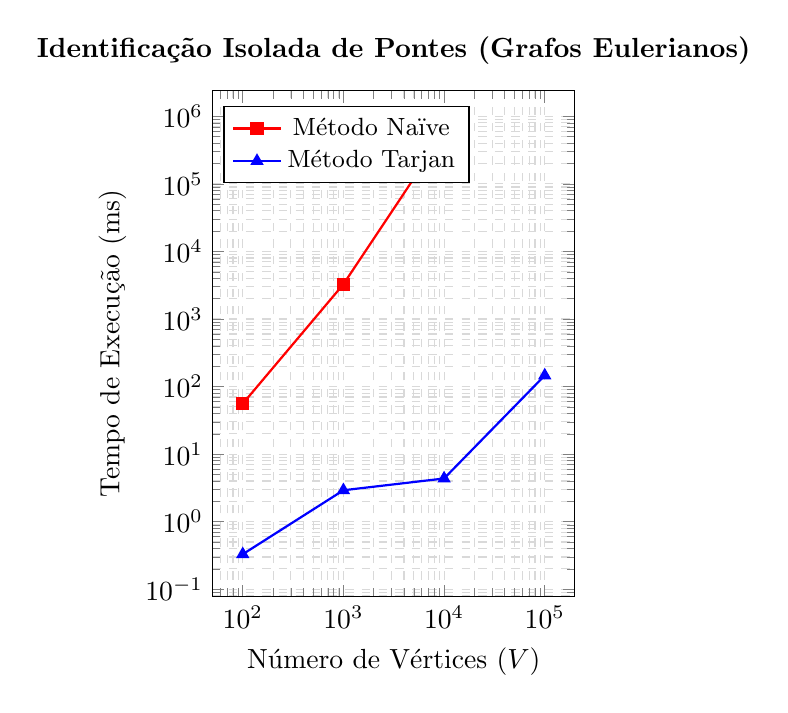
\begin{tikzpicture}
        \begin{axis}[
            width=0.51\textwidth,
            height=8cm,
            xmode=log, % Eixo X em escala logarítmica
            ymode=log, % Eixo Y em escala logarítmica
            title={\textbf{Identificação Isolada de Pontes (Grafos Eulerianos)}},
            xlabel={Número de Vértices ($V$)},
            ylabel={Tempo de Execução (ms)},
            grid=both,
            grid style={dashed, gray!30},
            legend pos=north west,
            legend style={font=\small}
        ]
        
        % Dados do Método Naïve (Parou em 10.000)
        \addplot[color=red, mark=square*, thick] coordinates {
            
            (100, 55.76)
            (1000, 3271.27)
            (10000, 565143.88)
        };
        \addlegendentry{Método Naïve}

        % Dados do Método Tarjan (Foi até 100.000)
        \addplot[color=blue, mark=triangle*, thick] coordinates {
            
            (100, 0.33)
            (1000, 2.92)
            (10000, 4.36)
            (100000, 145.94)
        };
        \addlegendentry{Método Tarjan}
        
        \end{axis}
    \end{tikzpicture}
    \caption{Comparativo do tempo de execução para identificação de pontes. A escala logarítmica ilustra a complexidade exponencial/quadrática do Naïve contra a eficiência quase linear do Tarjan.}
    \label{fig:grafico_pontes}
\end{figure}

\begin{figure}[H]
    \centering
    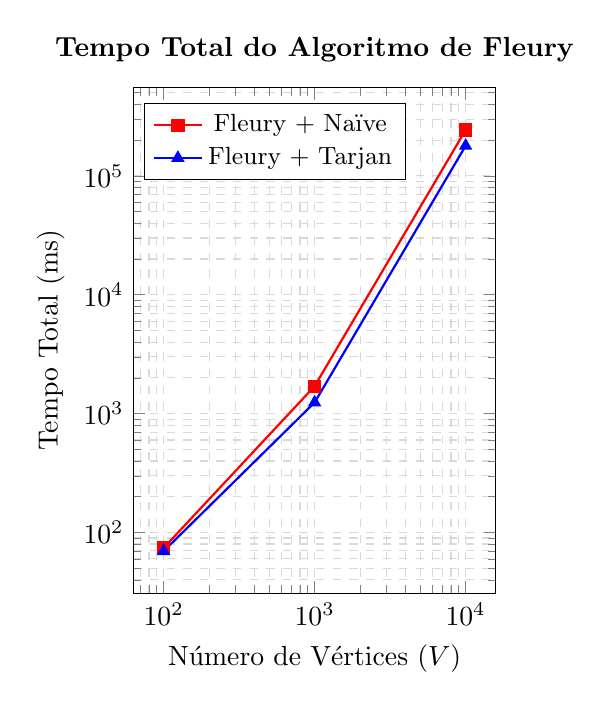
\begin{tikzpicture}
        \begin{axis}[
            width=0.51\textwidth,
            height=8cm,
            xmode=log,
            ymode=log,
            title={\textbf{Tempo Total do Algoritmo de Fleury}},
            xlabel={Número de Vértices ($V$)},
            ylabel={Tempo Total (ms)},
            grid=both,
            grid style={dashed, gray!30},
            legend pos=north west,
            legend style={font=\small}
        ]
        
        % Dados do Fleury + Naïve (Parou em 10.000)
        \addplot[color=red, mark=square*, thick] coordinates {
            
            (100, 74.17)
            (1000, 1702.51)
            (10000, 243172.12)
        };
        \addlegendentry{Fleury + Naïve}

        % Dados do Fleury + Tarjan (Parou em 10.000, pois >100k não terminou no log)
        \addplot[color=blue, mark=triangle*, thick] coordinates {
            
            (100, 69.73)
            (1000, 1241.13)
            (10000, 179051.29)
        };
        \addlegendentry{Fleury + Tarjan}
        
        \end{axis}
    \end{tikzpicture}
    \caption{Comparativo do tempo total do Algoritmo de Fleury executado sobre grafos Eulerianos. Nota-se que para grafos muito pequenos ($V=10$), o Fleury com Naïve otimizado tem vantagem por possuir menos \textit{overhead}, mas o Tarjan se torna superior conforme o tamanho do grafo escala.}
    \label{fig:grafico_fleury}
\end{figure}


\subsection{O "Timeout" dos 100k}

Durante a execução dos experimentos, observou-se que o algoritmo de Fleury~\citep{AlgoFleury} utilizando a abordagem Naive~\cite{cormen2022Naive} para a detecção de pontes não foi capaz de concluir sua execução dentro do limite de 12 horas para grafos de maior escala, especialmente para $V$ = 100.000 vértices. Para grafos com 10.000 vértices, o algoritmo ainda foi capaz de concluir a execução, embora com elevado tempo de processamento, sendo plenamente viável apenas até 1.000 vértices.

\subsubsection{Causa do "Timeout" na abordagem Naive}

A principal razão para esse desempenho insatisfatório está diretamente relacionada à forma como a abordagem Naive~\cite{cormen2022Naive} realiza a detecção de pontes. Para verificar se uma aresta é uma ponte, o método Naive~\cite{cormen2022Naive} executa os seguintes passos:

    \begin{itemize}
        \item Remove temporariamente a aresta do grafo;
        \item Executa uma busca completa para verificar se o grafo permanece conexo;
        \item Restaura a aresta removida.
    \end{itemize}

Esse procedimento é computacionalmente custoso, pois a cada verificação é necessário percorrer grande parte do grafo.

\subsubsection{Complexidade da abordagem Naive}

Cada verificação de ponte possui custo: 
$$O(V + E)$$
No entanto, durante a execução do algoritmo de Fleury~\citep{AlgoFleury} , essa verificação é realizada repetidamente, potencialmente para diversas arestas ao longo do processo. Dessa forma, a complexidade total aproximada torna-se:
$$O(E \cdot (V + E))$$
Para grafos grandes, como os de 100.000 vértices, esse custo se torna proibitivo, levando a tempos de execução extremamente elevados e, consequentemente, ao timeout observado.

\subsubsection{Abordagem com o algoritmo de Tarjan}

Em contraste, a versão otimizada utiliza o algoritmo de Tarjan~\cite{tarjan1972dfs} para identificação de pontes.

O algoritmo de Tarjan~\cite{tarjan1972dfs} realiza essa tarefa por meio de uma única busca em profundidade (DFS), calculando informações auxiliares (como tempos de descoberta e valores de menor alcance) para identificar todas as pontes do grafo de forma eficiente.

\subsubsection{Complexidade da abordagem Tarjan}

A detecção de pontes com Tarjan~\cite{tarjan1972dfs} possui complexidade:
$$O(V + E)$$
Ou seja, todas as pontes são encontradas em uma única passagem pelo grafo, eliminando a necessidade de múltiplas verificações custosas.

\subsubsection{Comparação de desempenho}

Os resultados experimentais evidenciam claramente a diferença entre as abordagens:

\begin{table}[H] % Mantenha o [H] para forçar o lugar
\centering
\caption{Comparativo de Desempenho: Fleury Naive vs. Fleury + Tarjan}
\label{tab:comparativo_algoritmos}
\resizebox{\columnwidth}{!}{ % Começa o redimensionamento
    \begin{tabular}{|l|c|c|}
    \hline
    \textbf{Nº de Vértices} & \textbf{Fleury + Naive} & \textbf{Fleury + Tarjan} \\ \hline
    100                     & Executa corretamente & Executa corretamente    \\ \hline
    1.000                   & Executa corretamente & Executa corretamente    \\ \hline
    10.000                  & Executa corretamente & Executa corretamente    \\ \hline
    100.000                 & \textit{Timeout} (> 12h) & 6 a 8 horas             \\ \hline
    \end{tabular}
} % Fecha o resizebox
\end{table}

A Tabela ~\ref{tab:comparativo_algoritmos} evidencia de forma clara o impacto da estratégia de detecção de pontes no desempenho do algoritmo de Fleury~\citep{AlgoFleury}. Observa-se que, para grafos de menor escala (até 10.000 vértices), ambas as abordagens são capazes de concluir a execução, embora a versão Naive~\cite{cormen2022Naive} apresente maior custo computacional. Entretanto, à medida que o tamanho do grafo cresce, a diferença de desempenho torna-se significativa. Para grafos com 100.000 vértices, a abordagem Naive~\cite{cormen2022Naive} torna-se inviável, não sendo capaz de finalizar a execução dentro do limite de 12 horas, enquanto a versão utilizando o algoritmo de Tarjan~\cite{tarjan1972dfs}, embora ainda custosa, consegue concluir em um intervalo entre 6 e 8 horas. Esses resultados demonstram, na prática, a superioridade da abordagem baseada em Tarjan~\cite{tarjan1972dfs} em termos de escalabilidade.


\section{Conclusão}

O presente trabalho teve como objetivo principal comparar a eficiência de duas abordagens para identificação de pontes em grafos, o método Naive~\cite{cormen2022Naive} e o algoritmo de Tarjan~\cite{tarjan1972dfs} quando integradas ao algoritmo de Fleury~\cite{AlgoFleury} para a determinação de caminhos eulerianos. A análise foi conduzida considerando grafos simples, não direcionados e conexos, com diferentes classificações (eulerianos, semi-eulerianos e não eulerianos) e múltiplas escalas de tamanho.

Os resultados experimentais apresentados nas Tabelas \ref{tab:pontes_isoladas}, \ref{tab:fleury_integrado} e \ref{tab:comparativo_algoritmos}, bem como nas Figuras \ref{fig:grafico_pontes} e \ref{fig:grafico_fleury}, evidenciam de forma clara a superioridade do algoritmo de Tarjan~\cite{tarjan1972dfs} em termos de desempenho e escalabilidade. Enquanto a abordagem Naive~\cite{cormen2022Naive} apresentou tempos de execução significativamente elevados já a partir de grafos com 10.000 vértices, tornando-se inviável para grafos com 100.000 vértices (não concluindo a execução dentro do limite de 12 horas), o algoritmo de Tarjan~\cite{tarjan1972dfs} foi capaz de processar todas as instâncias, ainda que com custo elevado para a maior escala, concluindo em aproximadamente 6 a 8 horas.

Essa diferença de desempenho está diretamente relacionada às complexidades computacionais das abordagens. O método Naive~\cite{cormen2022Naive}, ao verificar a conectividade do grafo a cada remoção de aresta, apresenta complexidade aproximada de $O(E⋅(V+E))$, o que se torna proibitivo para grafos de grande porte. Em contraste, o algoritmo de Tarjan~\cite{tarjan1972dfs} realiza a identificação de todas as pontes em uma única travessia do grafo, com complexidade $O(V+E)$, o que explica sua maior velocidade e eficiência prática.

Observa-se ainda que, para grafos de pequeno porte (como $V$ = 100), ambas as abordagens são viáveis, embora o método Naive~\cite{cormen2022Naive} já apresente maior custo computacional. À medida que o tamanho do grafo cresce, essa diferença torna-se cada vez mais significativa, impactando diretamente o desempenho do algoritmo de Fleury~\cite{AlgoFleury} como um todo.

Dessa forma, os resultados experimentais confirmam a expectativa teórica de que a escolha de um método mais eficiente para a identificação de pontes influencia decisivamente o desempenho global do algoritmo. Na prática, isso evidencia a importância da seleção adequada de algoritmos e estruturas de dados, especialmente em problemas que envolvem grandes volumes de dados.

\section*{Declarations}

\begin{contributions}
Aisha Camille foi responsável pela integração do Algoritmo de Fleury, criação do sistema de registro de dados (Logger) para melhor registro dos resultados dos algortimos. Iuri Saad implementou a estrutura de dados do Grafo e o gerador de instâncias. Mateus Brant foi responsável pela implementação dos métodos de identificação de pontes (Naïve e Tarjan). Todos os autores revisaram e aprovaram a versão final do relatório.
\end{contributions}

\begin{interests}
Os autores declaram que não possuem conflitos de interesse.
\end{interests}


\begin{materials}
Os códigos-fonte em Java desenvolvidos e os conjuntos de dados gerados durante os experimentos estão abertamente disponíveis no repositório GitHub através do link: [https://github.com/saadiuri/Trabalhos-Grafos.git]
\end{materials}


\bibliographystyle{ieeetr}
\bibliography{refs}

\end{document}
